\documentclass[border=0.125cm]{standalone}
\usepackage{tikz}
\usepackage{pgfplots}
\usepackage{graphicx}

\usetikzlibrary{decorations.pathmorphing}
\pgfplotsset{compat=newest}
\usetikzlibrary{shapes.geometric,arrows,fit,matrix,positioning}
\tikzset{main node/.style={circle,fill=black!20,draw,minimum size=3.5mm,inner sep=0pt},
         every node/.style={circle,fill=black,draw,minimum size=1mm,inner sep=0pt,label distance=-1mm},
         subtree/.style={isosceles triangle,fill=black!20,draw,minimum size=5mm,inner sep=0pt,shape border rotate=90},
         edge label/.style = {rectangle,draw=none,fill=none},
         blank edge/.style={edge from parent/.style={draw=none}},
         norm edge/.style={edge from parent/.style={black,thin,draw}},
}
\begin{document}
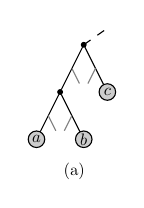
\begin{tikzpicture}[-,>=stealth', 
level 1/.style={sibling distance = 10mm},
level distance = 1cm, 
scale=0.6,
transform shape]
% \draw[help lines] (-2,0) grid (5,-5);
\node (1) {}
    child[norm edge]{
        node (2) {}
        child{ node [main node] (4) {$a$}}
        child{ node [main node] (5) {$b$}}
    }
    child[norm edge]{
        node [main node] (3) {$c$}
    }
;

\node[edge label,xshift=-2mm,below=25mm] at (1) {(a)};

\draw[gray] (0.25,-0.5) -- (0.09,-0.82);
\draw[gray] (-0.25,-0.5) -- (-0.09,-0.82);
\draw[gray] (-0.25,-1.5) -- (-0.41,-1.82);
\draw[gray] (-0.75,-1.5) -- (-0.59,-1.82);
\draw[dashed] (0,0) -- (0.5,0.35);   
\end{tikzpicture}
~~~~
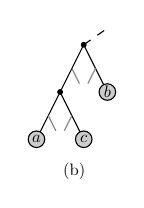
\begin{tikzpicture}[-,>=stealth', 
level 1/.style={sibling distance = 10mm},
level distance = 1cm, 
scale=0.6,
transform shape]
% \draw[help lines] (-2,0) grid (5,-5);
\node (1) {}
    child[norm edge]{
        node (2) {}
        child{ node [main node] (4) {$a$}}
        child{ node [main node] (5) {$c$}}
    }
    child[norm edge]{
        node [main node] (3) {$b$}
    }
;
\node[edge label,xshift=-2mm,below=25mm] at (1) {(b)};
\draw[gray] (0.25,-0.5) -- (0.09,-0.82);
\draw[gray] (-0.25,-0.5) -- (-0.09,-0.82);
\draw[gray] (-0.25,-1.5) -- (-0.41,-1.82);
\draw[gray] (-0.75,-1.5) -- (-0.59,-1.82);
\draw[dashed] (0,0) -- (0.5,0.35);   
\end{tikzpicture}
~~~~
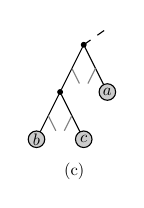
\begin{tikzpicture}[-,>=stealth', 
level 1/.style={sibling distance = 10mm},
level distance = 1cm, 
scale=0.6,
transform shape]
% \draw[help lines] (-2,0) grid (15,-15);
\node (1) {}
    child[norm edge]{
        node (2) {}
        child{ node [main node] (4) {$b$}}
        child{ node [main node] (5) {$c$}}
    }
    child[norm edge]{
        node [main node] (3) {$a$}
    }
;
\node[edge label,xshift=-2mm,below=25mm] at (1) {(c)};
\draw[gray] (0.25,-0.5) -- (0.09,-0.82);
\draw[gray] (-0.25,-0.5) -- (-0.09,-0.82);
\draw[gray] (-0.25,-1.5) -- (-0.41,-1.82);
\draw[gray] (-0.75,-1.5) -- (-0.59,-1.82);
\draw[dashed] (0,0) -- (0.5,0.35);   
\end{tikzpicture}

\end{document}



















